% PDF companion to ../ARCHITECTURE.md. Regenerate with:
% pdflatex -interaction=nonstopmode -halt-on-error -output-directory docs docs/ARCHITECTURE.tex
\documentclass[11pt]{article}
\usepackage[margin=0.8in]{geometry}
\usepackage[T1]{fontenc}
\usepackage[utf8]{inputenc}
\usepackage{lmodern}
\usepackage{xcolor}
\usepackage{hyperref}
\usepackage{tikz}
\usetikzlibrary{arrows.meta,positioning,shapes.geometric}

\hypersetup{
  colorlinks=true,
  linkcolor=blue!50!black,
  urlcolor=blue!50!black,
  pdftitle={Control Tower architecture},
  pdfauthor={TCP Group}
}

\tikzset{
  component/.style={draw=blue!60!black, rounded corners=3pt, fill=blue!6,
    minimum width=2.35cm, minimum height=0.85cm, align=center},
  database/.style={draw=gray!70!black, rounded corners=5pt, fill=gray!12,
    minimum width=2.35cm, minimum height=0.85cm, align=center},
  flow/.style={-{Stealth[length=2mm]}, thick, gray!70!black},
  bidirectional/.style={<->, thick, gray!70!black}
}

\begin{document}

\begin{center}
  {\LARGE\bfseries Control Tower architecture}\par\vspace{0.35em}
  \small PDF companion to \href{https://github.com/gaston-lm/tcp-nextwave-hackathon/blob/main/ARCHITECTURE.md}{ARCHITECTURE.md}
\end{center}

\vspace{0.8em}
\begin{center}
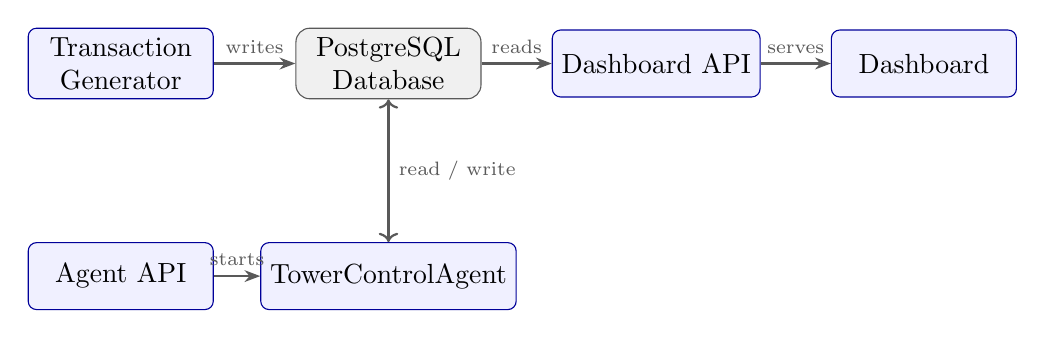
\begin{tikzpicture}
  \node[component] (generator) at (0, 1.4) {Transaction\\Generator};
  \node[database] (postgres) at (3.4, 1.4) {PostgreSQL\\Database};
  \node[component] (dashboardapi) at (6.8, 1.4) {Dashboard API};
  \node[component] (dashboard) at (10.2, 1.4) {Dashboard};

  \node[component] (agentapi) at (0, -1.3) {Agent API};
  \node[component] (tower) at (3.4, -1.3) {TowerControlAgent};

  \draw[flow] (generator) -- node[above, font=\scriptsize] {writes} (postgres);
  \draw[flow] (postgres) -- node[above, font=\scriptsize] {reads} (dashboardapi);
  \draw[flow] (dashboardapi) -- node[above, font=\scriptsize] {serves} (dashboard);
  \draw[flow] (agentapi) -- node[above, font=\scriptsize] {starts} (tower);
  \draw[bidirectional] (tower) -- node[right, font=\scriptsize] {read / write} (postgres);
\end{tikzpicture}
\end{center}

\section*{Components}

\begin{itemize}
  \item \href{https://github.com/gaston-lm/tcp-nextwave-hackathon/blob/main/scripts/ingestion/generator/README.md}{\textbf{Transaction Generator}} produces synthetic payment transactions and writes them to PostgreSQL.
  \item \href{https://github.com/gaston-lm/tcp-nextwave-hackathon/blob/main/data/README.md}{\textbf{PostgreSQL}} is the shared system of record for transactions, baseline metrics, and incidents.
  \item \href{https://github.com/gaston-lm/tcp-nextwave-hackathon/blob/main/services/dashboard_api/README.md}{\textbf{Dashboard API}} reads operational data from PostgreSQL and exposes it to the dashboard.
  \item \href{https://github.com/gaston-lm/tcp-nextwave-hackathon/blob/main/apps/dashboard/README.md}{\textbf{Dashboard}} displays payment activity and incidents through the Dashboard API.
  \item \href{https://github.com/gaston-lm/tcp-nextwave-hackathon/blob/main/services/agent_api/README.md}{\textbf{Agent API}} starts the investigation workflow.
  \item \textbf{TowerControlAgent} is the multi-agent orchestration that reads investigation context from PostgreSQL and writes the resulting operational records. See the \href{https://github.com/gaston-lm/tcp-nextwave-hackathon/blob/main/services/agent_api/README.md#orchestration}{detailed agent and tool orchestration}.
\end{itemize}

\end{document}
